\section{需求验证}

\subsection{验证与确认}

\subsubsection{概念引入}
需求验证:以正确的方式建立需求
\vspace{-0.8em}
\begin{multicols}{2}
    \begin{itemize}
        \item 需求集是正确的、完备的和一致的
        \item 技术上是可解决的
        \item 它们在现实世界中的满足是可行的和可验证的
    \end{itemize}
\end{multicols}
\vspace{-1em}

需求确认:建立的需求是正确的
\begin{itemize}
    \item 每一条需求都是符合用户原意的
\end{itemize}

\subsubsection{需求验证活动}
和验证活动贯穿于软件开发活动一样,验证活动同样也普遍存在于需求开发活动中。例如:
\begin{itemize}
    \item 在需求获取中:获得的用户需求是否正确和充分的支持业务需求?
    \item 在需求分析中:建立的分析模型是否正确的反映了问题域特性和需求?细化的系统需求是否充分和正确的支持用户需求?
    \item 需求规格说明:需求规格说明文档是否组织良好、书写正确?需求规格说明文档内的需求是否充分和正确的反映了涉众的意图?需求规格说明文档是否可以作为后续开发工作(设计、实现、测试等等)的基础? 
\end{itemize}

本章所述的需求验证是专指在需求规格说明完成之后,对需求规格说明文档进行的验证活动

\begin{figure}[H]
    \centering
    \vspace{-0.2em}
	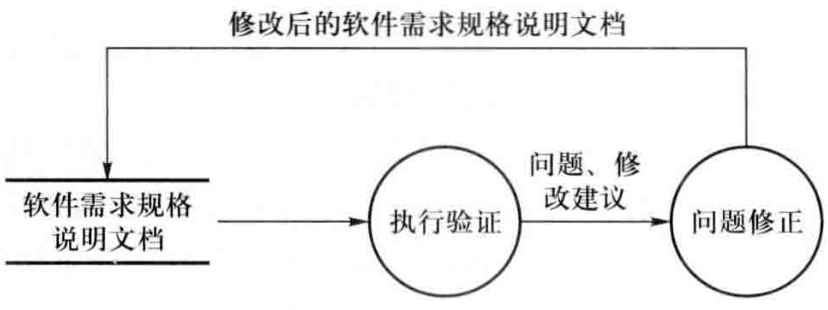
\includegraphics[width=0.6\textwidth]{img/需求验证活动流程图.png}
    \caption*{需求验证活动流程图}
    \vspace{-1em}
\end{figure}


\subsection{需求验证方法}

\subsubsection{需求评审}
评审又被称为同级评审,是指由作者之外的其他人来检查产品问题。在系统验证当中,评审是主要的静态分析手段,所以评审也是需求评审的一种主要方法。原则上,每一条需求都应该进行评审。

\begin{figure}[H]
	\setcounter{subfigure}{0}
	\centering
	\vspace{-0.5em}	
	\subfloat[同级评审的参与人员]{
		\begin{minipage}[t]{0.48\linewidth}
		\centering
		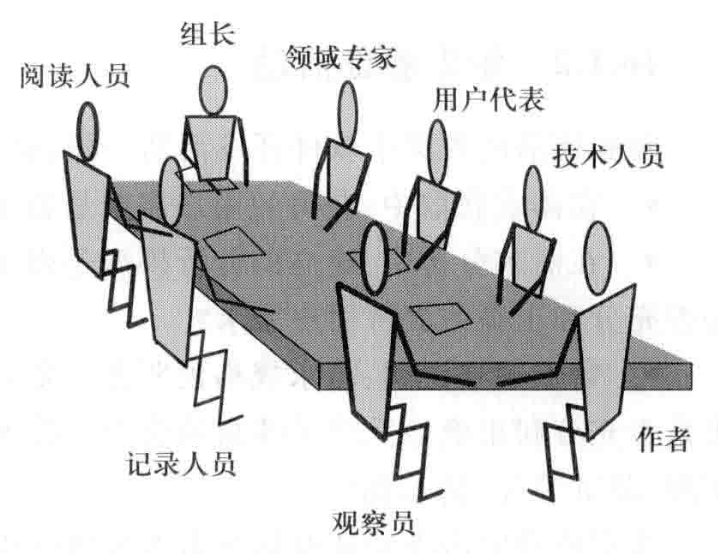
\includegraphics[width=0.9\linewidth]{img/同级评审的参与人员.png}
		\end{minipage}
	}
    \hfill
	\subfloat[同级评审的过程]{
		\begin{minipage}[t]{0.48\linewidth}
		\centering
		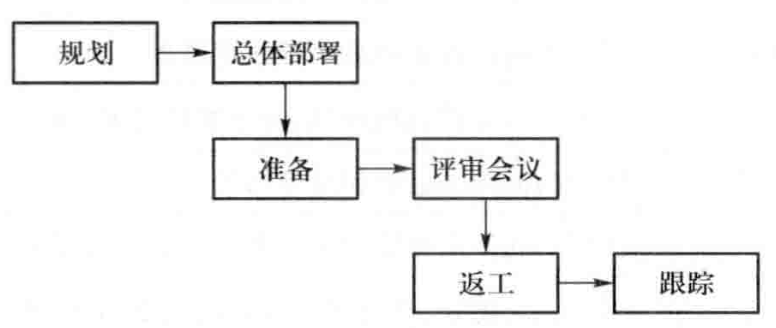
\includegraphics[width=\linewidth]{img/同级评审的过程.png}
		\end{minipage}
	}
	\centering
	\vspace{-1em}
\end{figure}

常见的评审的检查方法如下


\vspace{-0.8em}
\begin{center}
\begin{longtable}{|m{3cm}<{\centering}|m{8.5cm}|}
    \hline
    检查方法                       & \multicolumn{1}{c|}{描述}                                                                    \\ \hline
    自由方法(Ad-hoc)               & 没有为检查人员提供系统化的引导                                                       \\ \hline
    检查清单(Checklist-Based)      & 以通用的检查清单来引导检查过程                                                       \\ \hline
    缺陷(Defect-Based)           & 用于需求文档,根据缺陷的分类来组织和检查场景                                                \\ \hline
    功能点(Function Point-Based)  & 按照功能点来组织和检查场景                                                         \\ \hline
    视角(Perspective-Based)      & 按照不同涉众类型的视角来组织和检查场景                                                   \\ \hline
    场景(Scenario-Based)         & 对每一个场景,都利用一系列的问题或者细节要求,来引导检查过程。缺陷、功能点、视角都是场景方法的一个特例。                  \\ \hline
    逐步提升(Stepwise Abstraction) & 净室软件开发中的一种方法。阅读者描述一些独立代码段的功能,然后将描述的范围逐步扩大,描述的功能抽象逐步提高,直至阅读人员描述了整个评审物件 \\ \hline
\end{longtable}
\end{center}
\vspace{-3.7em}

[Wiegers 2002]对评审类型的分类如下图所示
\begin{figure}[H]
    \centering
    \vspace{-0.2em}
	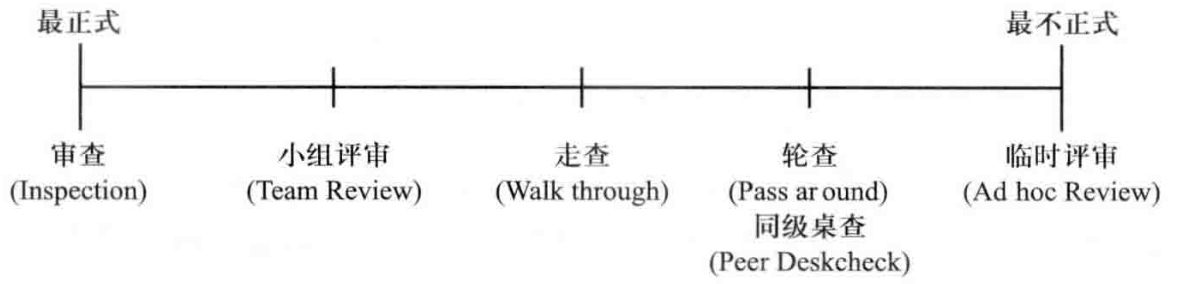
\includegraphics[width=0.8\textwidth]{img/评审的类型.png}
    \caption*{评审的类型}
    \vspace{-1em}
\end{figure}


\subsubsection{原型与模拟}
当有些需求涉及复杂的动态行为时,它可能就需要使用原型或模拟方法来加以验证。该方法成本较高。
\begin{figure}[H]
    \centering
    \vspace{-0.2em}
	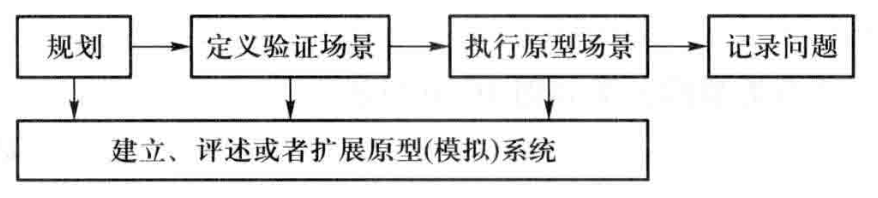
\includegraphics[width=0.65\textwidth]{img/利用原型和模拟进行需求验证的过程.png}
    \caption*{利用原型和模拟进行需求验证的过程}
    \vspace{-1em}
\end{figure}


\subsubsection{开发测试用例}
在需求开发完成之后,测试人员就作为软件需求规格说明文档的读者开始进行测试计划。测试计划的主要活动是依据需求设计测试用例,这些测试用例将在软件系统实现之后的功能测试当中得到执行。在实践中发现,在为需求设计测试用例的过程当中可以发现软件需求规格说明文档的很多缺陷与问题。因此,为需求来开发测试用例也可以被看成一个有效的需求验证方法。

在这种需求验证方法下,要求为每个需求都开发测试用例。通常情况下,一条需求的满足可能需要很多个测试用例才能完全体现出来。同时,一个测试用例可能会被用来测试多条需求。如果无法为某条需求定义完备的测试用例,那么它可能就存在着模糊、信息遗漏、不正确等缺陷。

当然,无法定义测试用例的需求也并非是绝对有问题的。下列需求就是通常无法定义测试用例的。
\begin{itemize}
    \item 排斥性需求:这种需求要求特定的行为绝对不会发生,例如需求可能会要求系统故障不能导致数据库的崩溃
    \item 全局性非功能性需求:例如可靠性、可用性等,对这些需求的测试往往都是大数据集的处理
\end{itemize}

开发系统测试用例
\begin{itemize}
    \item 以需求为线索,开发测试用例套件
    \item 使用测试技术确定输入/输出数据,开发测试用例
\end{itemize}

测试用例套件:基于用例描述,可以为销售处理确定测试用例套件
\begin{table}[H]
    \centering
    \begin{tabular}{|c|cccccccc|}
    \hline
    测试用例套件 & \multicolumn{8}{c|}{覆盖流程}                                                                                                                                                             \\ \hline
    TUS1   & \multicolumn{1}{c|}{正常流程} & \multicolumn{1}{c|}{}   & \multicolumn{1}{c|}{3a} & \multicolumn{1}{c|}{3b} & \multicolumn{1}{c|}{5-8a} & \multicolumn{1}{c|}{}     & \multicolumn{1}{c|}{}   &     \\ \hline
    TUS2   & \multicolumn{1}{c|}{正常流程} & \multicolumn{1}{c|}{1a} & \multicolumn{1}{c|}{}   & \multicolumn{1}{c|}{}   & \multicolumn{1}{c|}{}     & \multicolumn{1}{c|}{}     & \multicolumn{1}{c|}{9a} & 11a \\ \hline
    TUS3   & \multicolumn{1}{c|}{正常流程} & \multicolumn{1}{c|}{}   & \multicolumn{1}{c|}{}   & \multicolumn{1}{c|}{}   & \multicolumn{1}{c|}{}     & \multicolumn{1}{c|}{5-8b} & \multicolumn{1}{c|}{}   &     \\ \hline
    \end{tabular}
    \vspace{-1em}
\end{table}


建立测试用例:主要是基于规格的技术,设计测试场景的输入与输出数据
\begin{table}[H]
    \centering
    \resizebox{\linewidth}{!}{
    \begin{tabular}{|l|llll|l|}
    \hline
    \multicolumn{1}{|c|}{\multirow{2}{*}{ID}} & \multicolumn{4}{c|}{输入}                                                                                                                                                                                                                & \multicolumn{1}{c|}{\multirow{2}{*}{预期输出}} \\ \cline{2-5}
    \multicolumn{1}{|c|}{}                    & \multicolumn{1}{c|}{商品信息}                                                                    & \multicolumn{1}{c|}{特价}                                                             & \multicolumn{1}{c|}{赠品} & \multicolumn{1}{c|}{支付} & \multicolumn{1}{c|}{}                      \\ \hline
    TUS1-1                                    & \multicolumn{1}{l|}{无商品}                                                                     & \multicolumn{1}{l|}{无}                                                              & \multicolumn{1}{l|}{无}  & 无                       & 不做任何处理,关闭销售任务                              \\ \hline
    TUS1-2                                    & \multicolumn{1}{l|}{\begin{tabular}[c]{@{}l@{}}商品1(1、1(双)、35)\\ 商品2(2、1(双)、50)\end{tabular}} & \multicolumn{1}{l|}{无}                                                              & \multicolumn{1}{l|}{无}  &                         &                                            \\ \hline
    TUS1-3                                    & \multicolumn{1}{l|}{\begin{tabular}[c]{@{}l@{}}商品1(1、1(双)、35)\\ 商品2(2、1(双)、50)\end{tabular}} & \multicolumn{1}{l|}{无}                                                              & \multicolumn{1}{l|}{无}  & 85                      & 无找零,系统行为满足后置条件                             \\ \hline
    TUS1-4                                    & \multicolumn{1}{l|}{\begin{tabular}[c]{@{}l@{}}商品1(1、1(双)、35)\\ 商品2(2、1(双)、50)\end{tabular}} & \multicolumn{1}{l|}{商品1特价20}                                                        & \multicolumn{1}{l|}{}   & 100                     & 找零30,系统行为满足后置条件                            \\ \hline
    TUS1-5                                    & \multicolumn{1}{l|}{\begin{tabular}[c]{@{}l@{}}商品1(1、1(双)、35)\\ 商品2(2、1(双)、50)\end{tabular}} & \multicolumn{1}{l|}{总额特价50以上0.8折}                                                   & \multicolumn{1}{l|}{}   & 100                     & 找零31,系统行为满足后置条件                            \\ \hline
    TUS1-6                                    & \multicolumn{1}{l|}{\begin{tabular}[c]{@{}l@{}}商品1(1、1(双)、35)\\ 商品2(2、1(双)、60)\end{tabular}} & \multicolumn{1}{l|}{\begin{tabular}[c]{@{}l@{}}商品1特价20\\ 总额特价50以上0.8折\end{tabular}} & \multicolumn{1}{l|}{}   & 100                     & 找零32,系统行为满足后置条件                            \\ \hline
    \end{tabular}
    }
    \vspace{-1em}
\end{table}


\subsubsection{用户手册编制}
用户手册主要包含以下内容
\vspace{-0.8em}
\begin{multicols}{2}
    \begin{itemize}
        \item 验证功能需求:对软件系统功能和实现的描述
        \item 验证项目范围:对系统没有实现的功能的描述
        \item 验证异常流程需求:问题和故障的解决
        \item 验证环境与约束需求:系统的安装和启动
    \end{itemize}
\end{multicols}
\vspace{-1em}


\subsubsection{利用跟踪关系}
业务需求$\rightarrow$用户需求$\rightarrow$系统需求
\begin{itemize}
    \item 如果业务需求和用户需求没有得到后项需求(用户需求和系统需求)的充分支持,那么软件需求规格说明文档就存在不完备的缺陷
\end{itemize}

系统需求$\rightarrow$用户需求$\rightarrow$业务需求
\begin{itemize}
    \item 如果不能依据跟踪关系找到一条系统需求的前项用户需求和前项业务需求,那么该需求就属于非必要的需求
\end{itemize}


\subsubsection{自动化分析}
自动化分析方法有一个非常强的限制前提——用形式化方法书写软件需求规格说明文档。因为形式化语言对用户而言难以理解,所以它较少使用。通常是对关键系统或系统的关键部分会进行形式化的描述,并使用自动化分析方法进行需求验证。

\begin{figure}[H]
    \centering
    \vspace{-0.2em}
	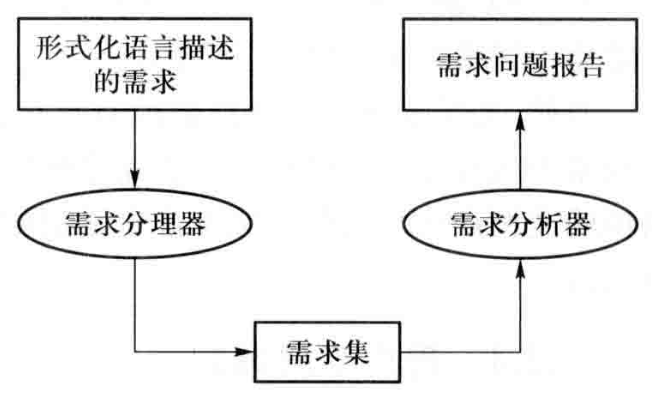
\includegraphics[width=0.41\textwidth]{img/需求文档的自动化分析.png}
    \caption*{需求文档的自动化分析}
    \vspace{-1em}
\end{figure}


\subsection{问题修正}
常见的问题修正行为有以下几种:
\vspace{-0.8em}
\begin{multicols}{2}
    \begin{itemize}
        \item 需求澄清
        \begin{itemize}
            \item 理解偏差:重新进行分析工作
            \item 分析遗漏:重新分析和文档化这部分信息
            \item 表达不当:重新以合适的方式表达
        \end{itemize}
        \item 缺失需求:重新执行需求获取等一系列工作
        \item 需求冲突:协商解决
        \item 不切实际的期望:项目调整与需求协商
    \end{itemize}
\end{multicols}
\vspace{-1em}

